\section{Industrialisation \& recul}

% ============================================================
% S17 — NeuralScope
% ============================================================
\begin{frame}{Industrialiser : NeuralScope}
  \framesubtitle{« Comprendre, corriger, piloter » : la recherche rendue utilisable}
  \begin{columns}[T,onlytextwidth]
    \column{0.52\textwidth}
      \centering
      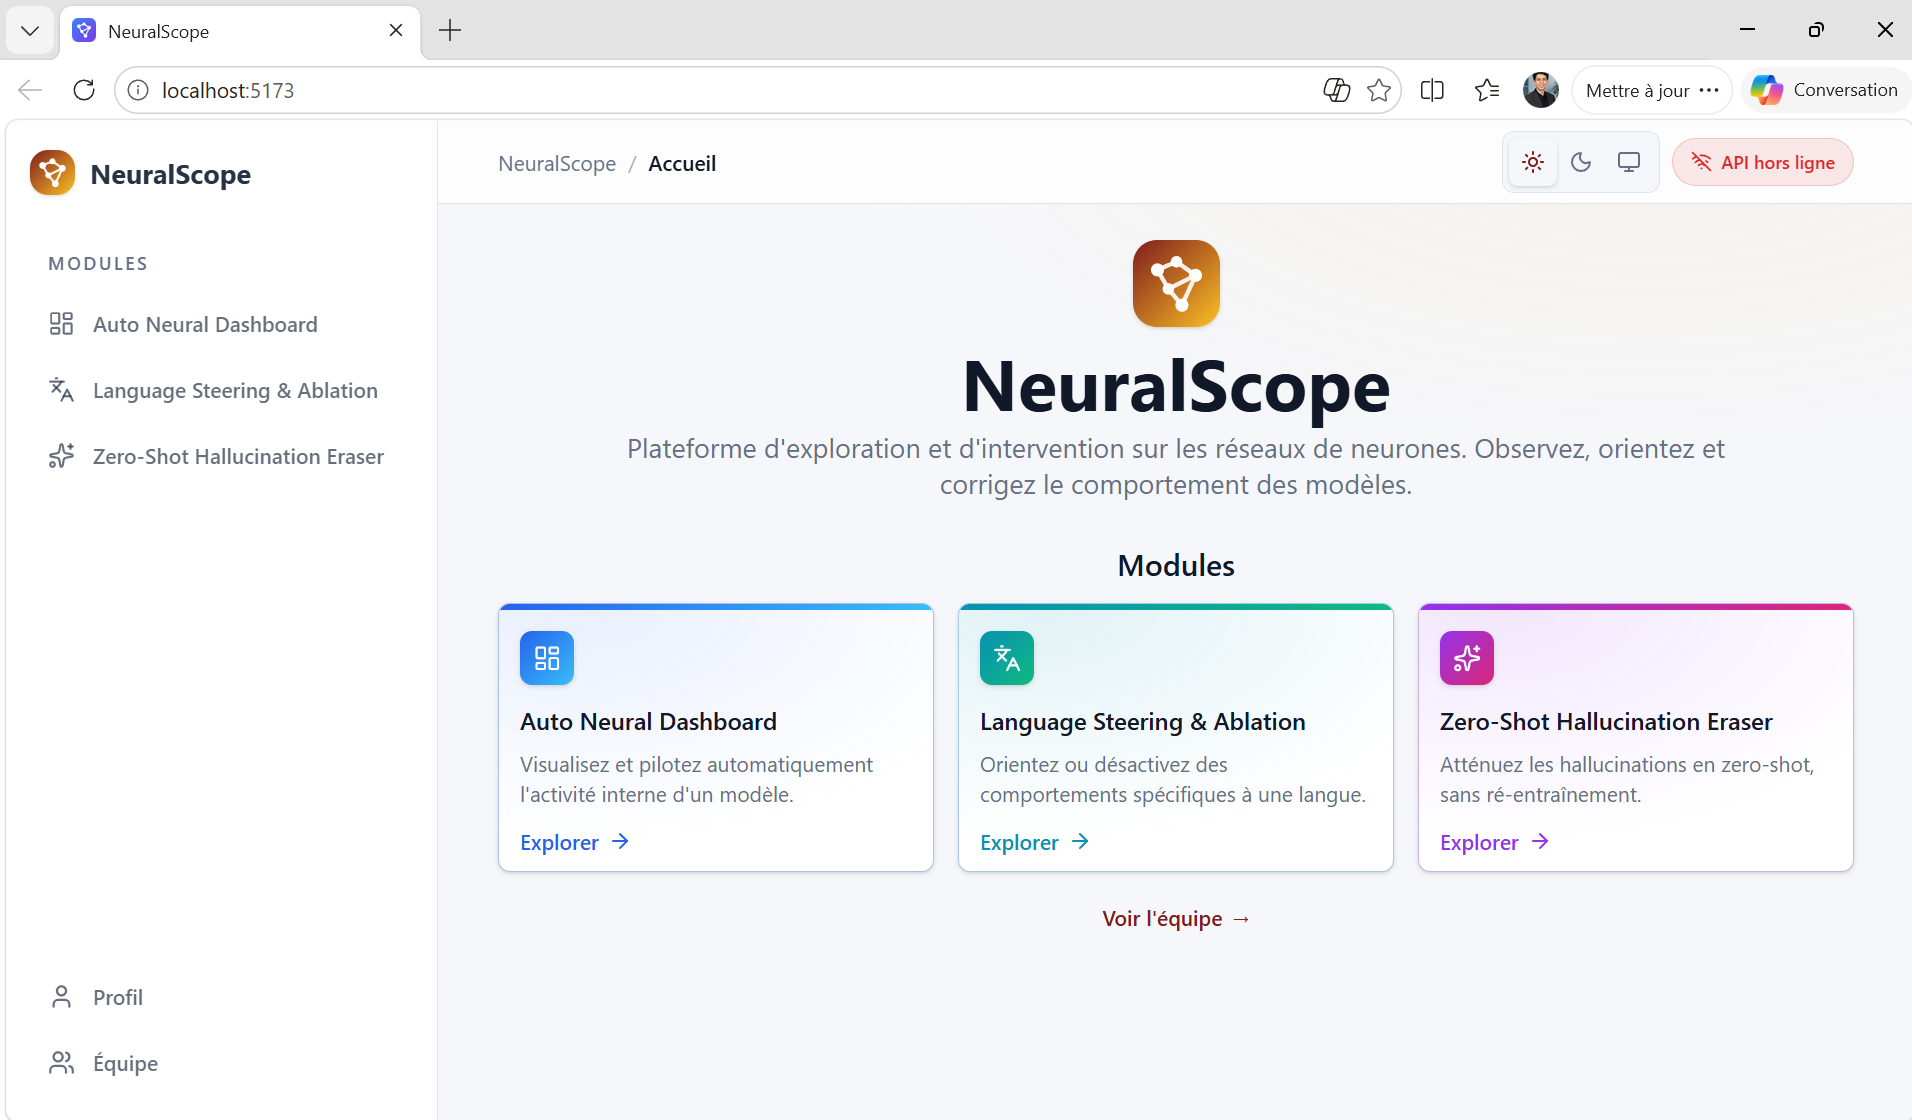
\includegraphics[width=\linewidth,height=0.62\textheight,keepaspectratio]{media/neuralscope_home.png}
    \column{0.44\textwidth}
      \begin{itemize}
        \item \small Plateforme unifiée des \textbf{3 PoC} de l'équipe EAI
        \item \small \textbf{Modular monolith} : une base déployable, modules hermétiques
        \item \small FastAPI / React TS / Docker
      \end{itemize}
      \begin{block}{Ma contribution}
        \footnotesize Module d'explicabilité complet : chargement modèle, génération, extraction NTP, entraînement des classifieurs.
      \end{block}
  \end{columns}
  \AubayTraceRef{A.5.2}
\end{frame}

% ============================================================
% S17bis — NeuralScope : deux modes, deux publics
% ============================================================
\begin{frame}{NeuralScope : deux modes, deux publics}
  \framesubtitle{Mode métier et mode développeur}
  \begin{columns}[T,onlytextwidth]
    \column{0.48\textwidth}
      \centering
      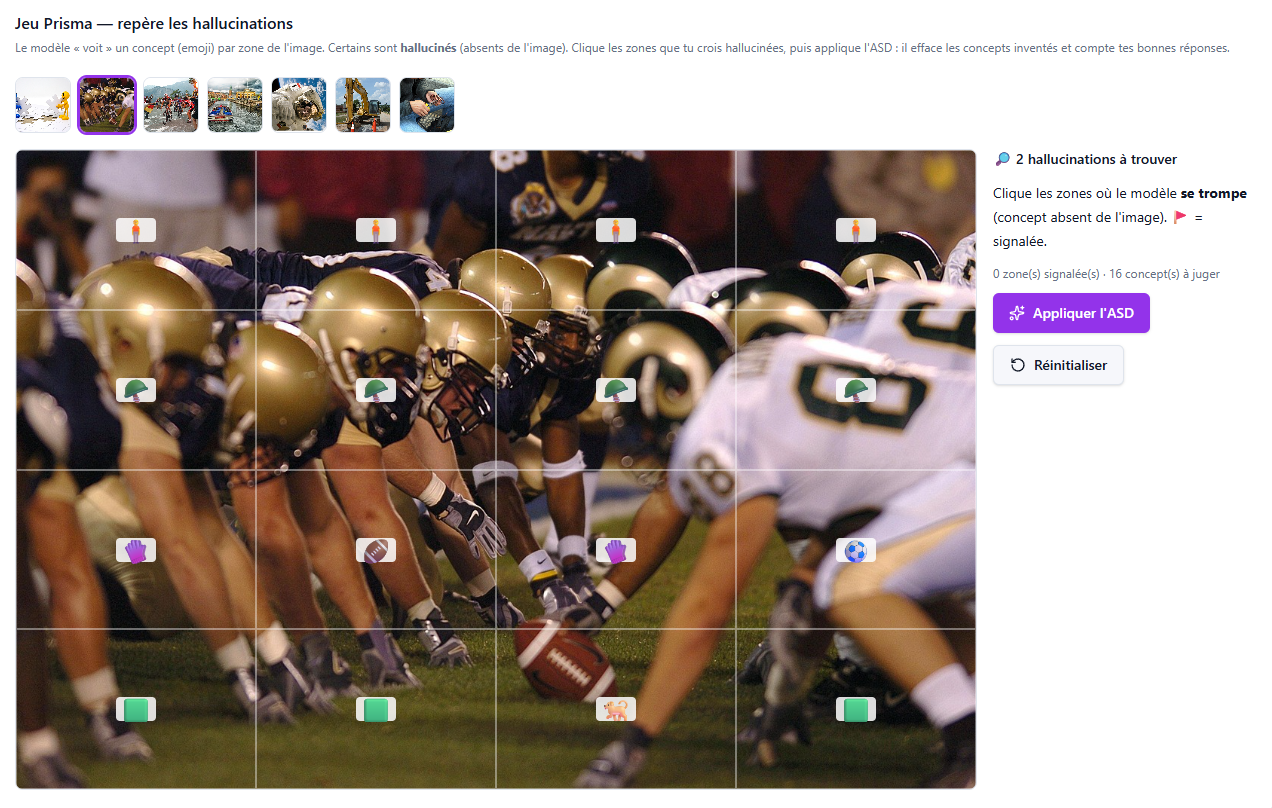
\includegraphics[width=\linewidth,height=0.48\textheight,keepaspectratio]{media/jeu_prisma.png}\par\vspace{0.1cm}
      \AubayStatusChip{AubayOrange}{MODE MÉTIER}\par\vspace{0.05cm}
      {\scriptsize jeu de détection · vues avant/après}
    \column{0.48\textwidth}
      \centering
      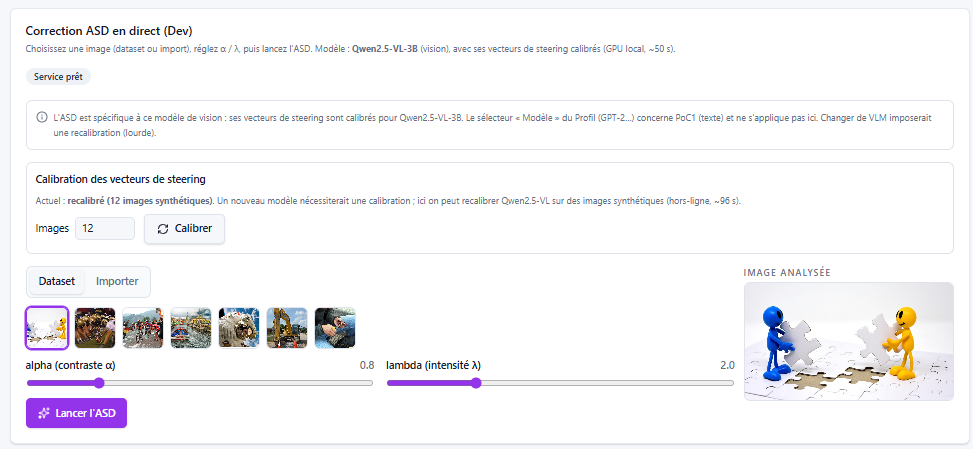
\includegraphics[width=\linewidth,height=0.48\textheight,keepaspectratio]{media/dev_mode.png}\par\vspace{0.1cm}
      \AubayStatusChip{AubayTeal}{MODE DÉVELOPPEUR}\par\vspace{0.05cm}
      {\scriptsize probabilités NTP · seuils ASD}
  \end{columns}
  \vspace{0.25cm}
  \centering
  \begin{minipage}{0.84\textwidth}
    \AubayFocusPanel{Valeur d'innovation}{Une \textbf{surcouche légère et réutilisable} : à brancher sur le VLM d'un client, sans réentraînement.}
  \end{minipage}
\end{frame}

% ============================================================
% S18 — Engagement éclairé du client
% ============================================================
\begin{frame}{Ce que je promets, et ce que je refuse de promettre}
  \framesubtitle{Un engagement client éclairé vaut mieux qu'une démo magique}
  \begin{columns}[T,onlytextwidth]
    \column{0.48\textwidth}
      \begin{exampleblock}{La solution promet}
        \small
        \begin{itemize}
          \item Un \textbf{signal de risque} phrase par phrase
          \item Coût marginal quasi nul (sous-produit de la génération)
          \item \textbf{100 \% local}: aucune donnée ne sort
          \item Zéro réentraînement du modèle client
        \end{itemize}
      \end{exampleblock}
    \column{0.48\textwidth}
      \begin{alertblock}{La solution ne promet pas}
        \small
        \begin{itemize}
          \item Une \textbf{garantie d'exactitude}
          \item Un déploiement sans \textbf{calibration métier} (cross-dataset !)
          \item Le remplacement de la revue humaine
        \end{itemize}
      \end{alertblock}
  \end{columns}
  \vspace{0.35cm}
  \centering
  \begin{minipage}{0.84\textwidth}
    \AubayFocusPanel{Posture défendue en comité}{Vendre un \textbf{outil de priorisation de la revue humaine}. Le jour où on le vend comme un label de vérité, on recrée le problème qu'on voulait résoudre.}
  \end{minipage}
\end{frame}

% ============================================================
% S19 — Ingénieur responsable : frugalité, local, accessibilité
% ============================================================
\begin{frame}{Des choix responsables : par conception, pas par affichage}
  \framesubtitle{Environnement, données, société : trois dispositifs concrets}
  \begin{columns}[T,onlytextwidth]
    \column{0.31\textwidth}
      \AubayPoCCard{IA frugale}{\AubayStatusChip{AubaySuccess}{ENVIRONNEMENT}}{dispositifs}{Modèles \textbf{256M -- 3B} choisis par benchmark · correction \textbf{à l'inférence}, zéro réentraînement · fallback CPU, quantification}
    \column{0.31\textwidth}
      \AubayPoCCard{100 \% local}{\AubayStatusChip{AubayTeal}{DONNÉES}}{dispositifs}{Aucun appel d'API cloud · images et sorties restent sur le poste · compatible données sensibles (KYC, santé)}
    \column{0.31\textwidth}
      \AubayPoCCard{Accessibilité}{\AubayStatusChip{AubayOrange}{SOCIÉTÉ}}{dispositifs}{Mode métier non technique + jeu pédagogique · perspective : description d'images fiable pour malvoyants}
  \end{columns}
  \vspace{0.4cm}
  \centering
  \AubayStatusChip{AubayOrange}{FRUGALITÉ ASSUMÉE, PAS SUBIE}\hspace{0.15cm}
  \AubayStatusChip{AubaySuccess}{POSTE CLIENT, PAS CLOUD}
  \AubayTraceRef{A.4.2}
\end{frame}
